% Chapter Template

\chapter{Ensayos y resultados} % Main chapter title

\label{Chapter4} % Change X to a consecutive number; for referencing this chapter elsewhere, use \ref{ChapterX}
\citep{ARTICLE:1}, \citep{BOOK:1}, \citep{BOOK:2}, \citep{WEBSITE:1}.

%----------------------------------------------------------------------------------------
%	SECTION 1
%----------------------------------------------------------------------------------------

\section{Pruebas funcionales del hardware}
\label{sec:pruebasHW}



\section{Pruebas de elección de canal y ancho de banda}


Los fundamentos y consideraciones para la mejoren la elección del canal y ancho de bana del canal Wi-Fi IoT que se usó, se describió en el ....capitulo 3 .... La elección dependió de las señales circundantes vecinas a la red domestica donde se instaló el sistema prototipo IoT. La figura.... muestra resultado del primer escaneo de las señales y el uso de los canales respectivos así como solapamiento existente entre ellos. 

De la imagen se describe lo siguiente:

\keyword{Señal WLAN IoT} 
\begin{itemize}
\item SSID: MATRIX-ICF
\item Canal: 10 (configuración automática)
\item Ancho de canal: 40 MHz (configuración automática)
\item Potencia señal: 93\%
\item Seguridad:  WPA2 (PSK)
\item Tasa Máxima de transferencia: 300 Mbps
\end{itemize}


\keyword{Señal WLAN doméstica}
\begin{itemize} 
\item SSID: CLARO-B612-D514
\item Canal: 11 (configuración automática)
\item Ancho de canal: 20 MHz (configuración automática)
\item Potencia señal: 64\%
\item Seguridad: WPA2 (PSK)
\item Tasa Máxima de transferencia: 144.4 Mbps
\end{itemize}

El procedimiento de mejora consistió en modificar la configuración por defecto del router/AP de la red IoT al cambiar el canal y reducir el ancho de banda, verificando en cada cambio el comportamiento de las señales en el ambiente y la reducción de solapamiento de los mismos.

%%%%%%%%%%%%%%%%%%%%%%%%%%%%%%%%%%%%%%%%%%%%%%%%%%%
\begin{landscape} % esto es para rotar la pagina e imagen
\begin{figure}[htpb]
\centering 
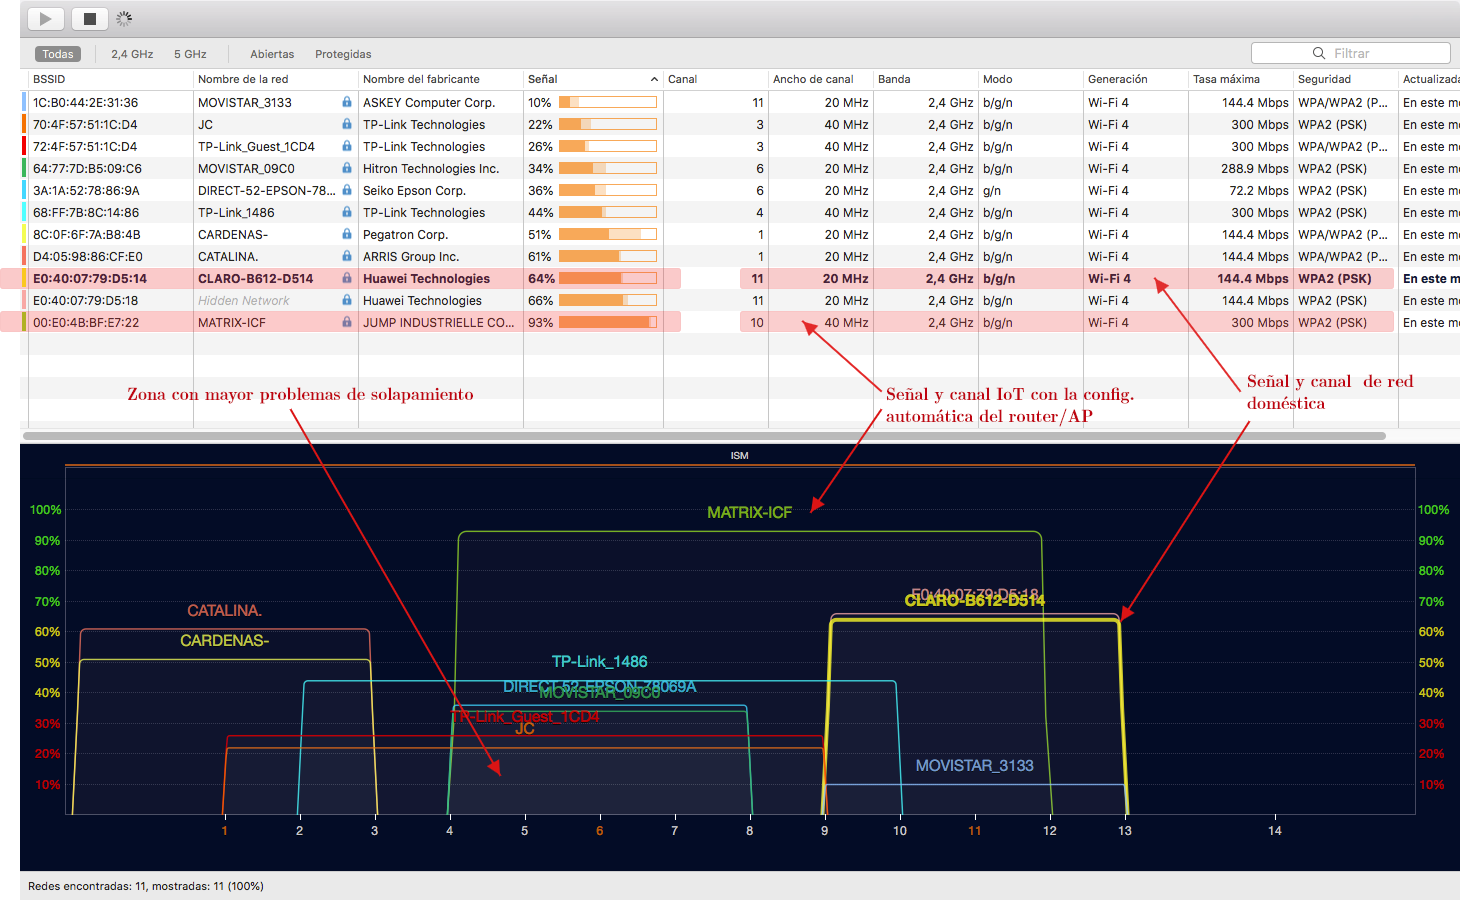
\includegraphics[width=1.5\textwidth]{./Figures/wifi/01.png}
\caption{..... .}
\label{fig:test01}
\end{figure}
\end{landscape} %

%%%%%%%%%%%%%%%%%%%%%%%%%%%%%%%%%%%%%%%%%%%%%%%%%%%

\begin{landscape} % esto es para rotar la pagina e imagen
\begin{figure}[htpb]
\centering 
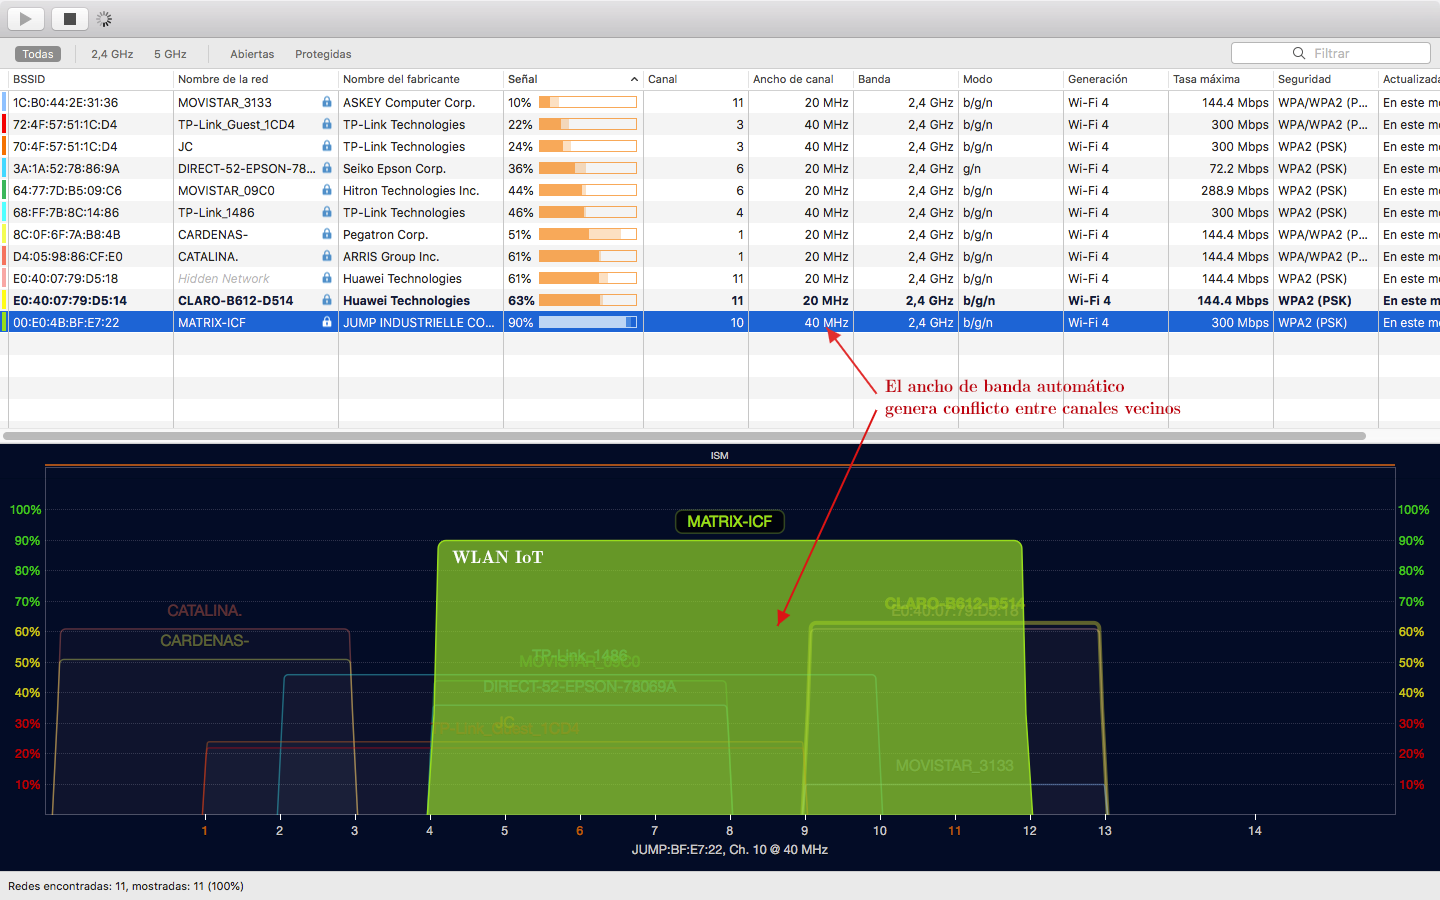
\includegraphics[width=1.5\textwidth]{./Figures/wifi/02.png}
\caption{..... .}
\label{fig:test02}
\end{figure}
\end{landscape} %


%%%%%%%%%%%%%%%%%%%%%%%%%%%%%%%%%%%%%%%%%%%%%%%%%%%
\begin{landscape} % esto es para rotar la pagina e imagen
\begin{figure}[htpb]
\centering 
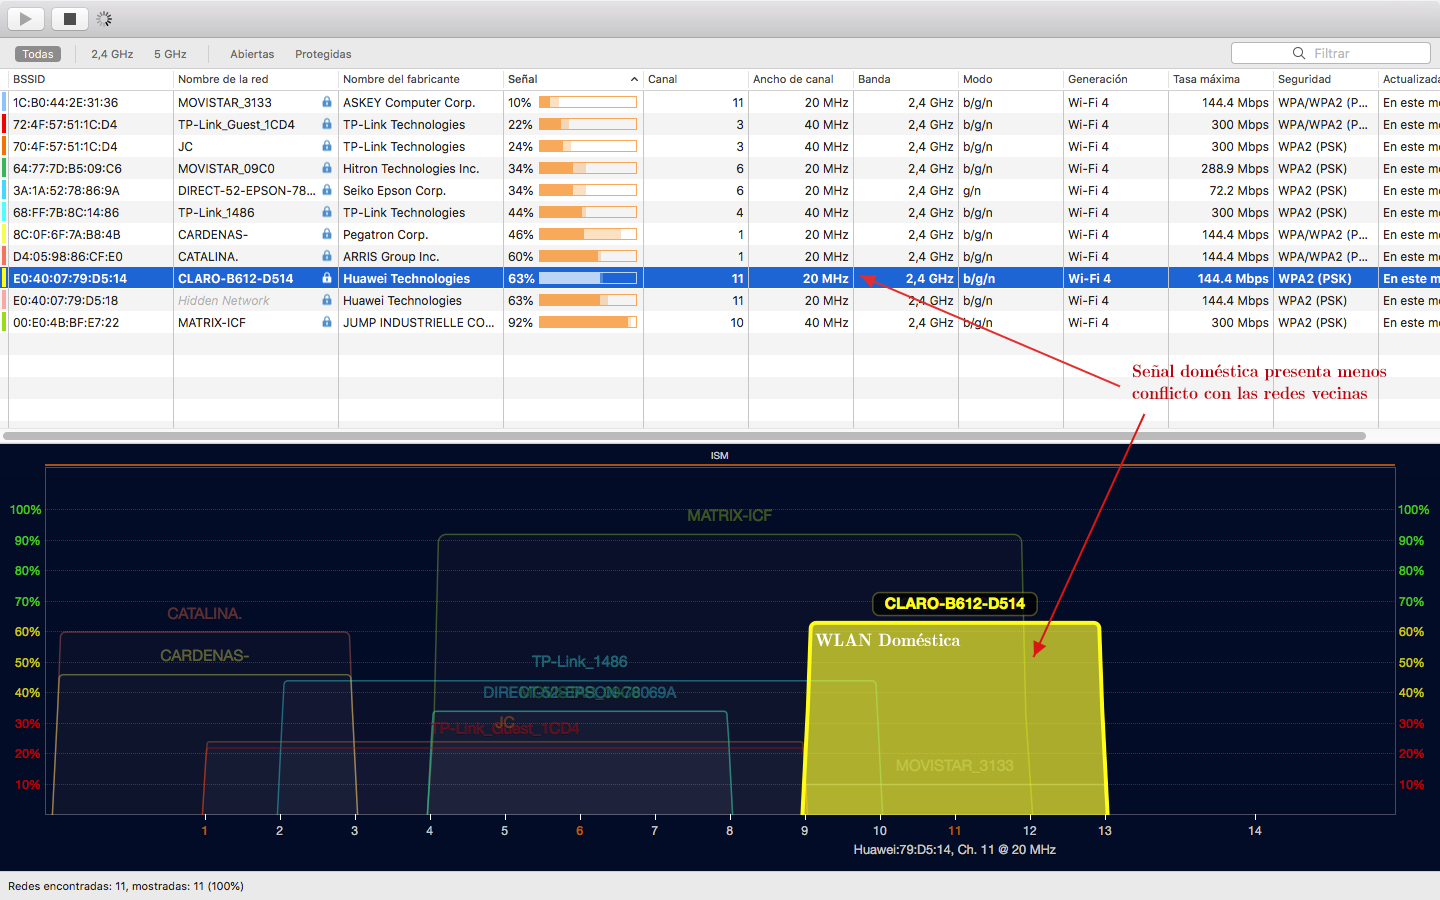
\includegraphics[width=1.5\textwidth]{./Figures/wifi/03.png}
\caption{..... .}
\label{fig:test03}
\end{figure}
\end{landscape} %

%%%%%%%%%%%%%%%%%%%%%%%%%%%%%%%%%%%%%%%%%%%%%%%%%%%

\begin{landscape} % esto es para rotar la pagina e imagen
\begin{figure}[htpb]
\centering 
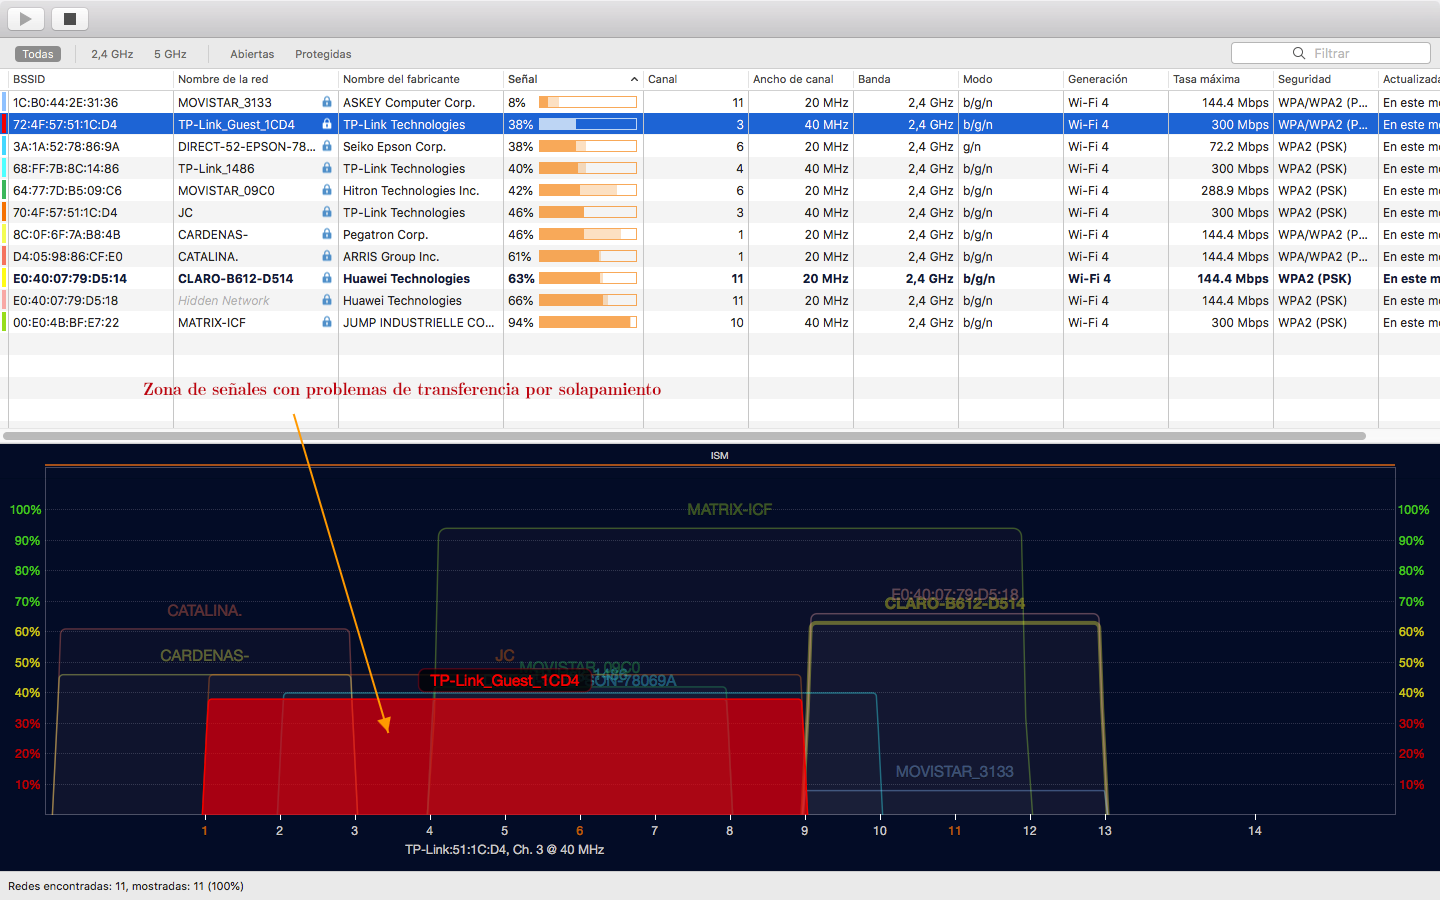
\includegraphics[width=1.5\textwidth]{./Figures/wifi/04.png}
\caption{..... .}
\label{fig:test04}
\end{figure}
\end{landscape} %


%%%%%%%%%%%%%%%%%%%%%%%%%%%%%%%%%%%%%%%%%%%%%%%%%%%

\begin{landscape} % esto es para rotar la pagina e imagen
\begin{figure}[htpb]
\centering 
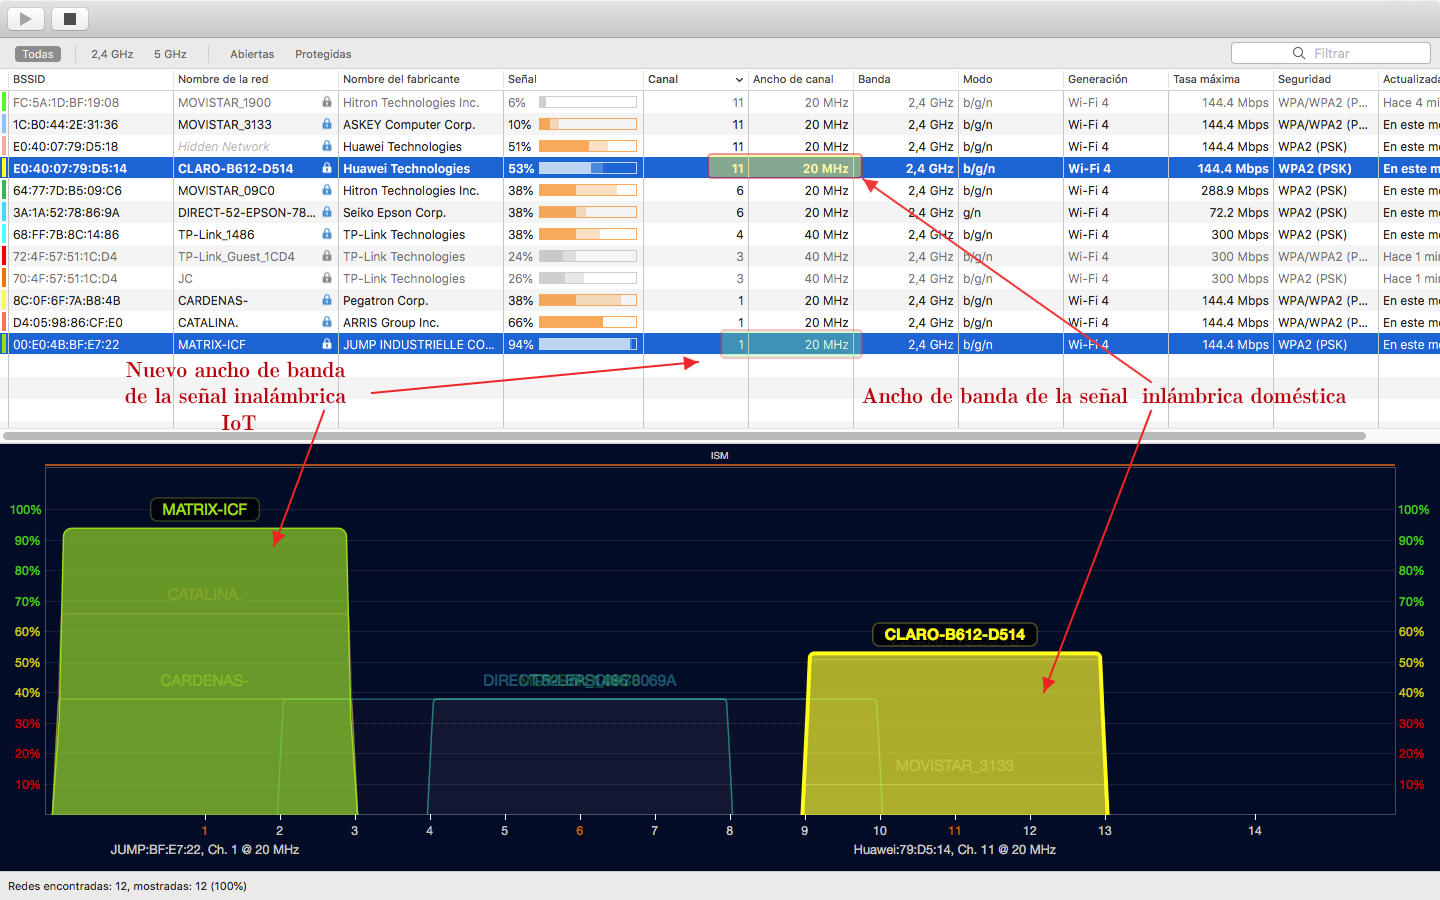
\includegraphics[width=1.5\textwidth]{./Figures/wifi/05.png}
\caption{..... .}
\label{fig:test05}
\end{figure}
\end{landscape} %


%%%%%%%%%%%%%%%%%%%%%%%%%%%%%%%%%%%%%%%%%%%%%%%%%%%

\begin{landscape} % esto es para rotar la pagina e imagen
\begin{figure}[htpb]
\centering 
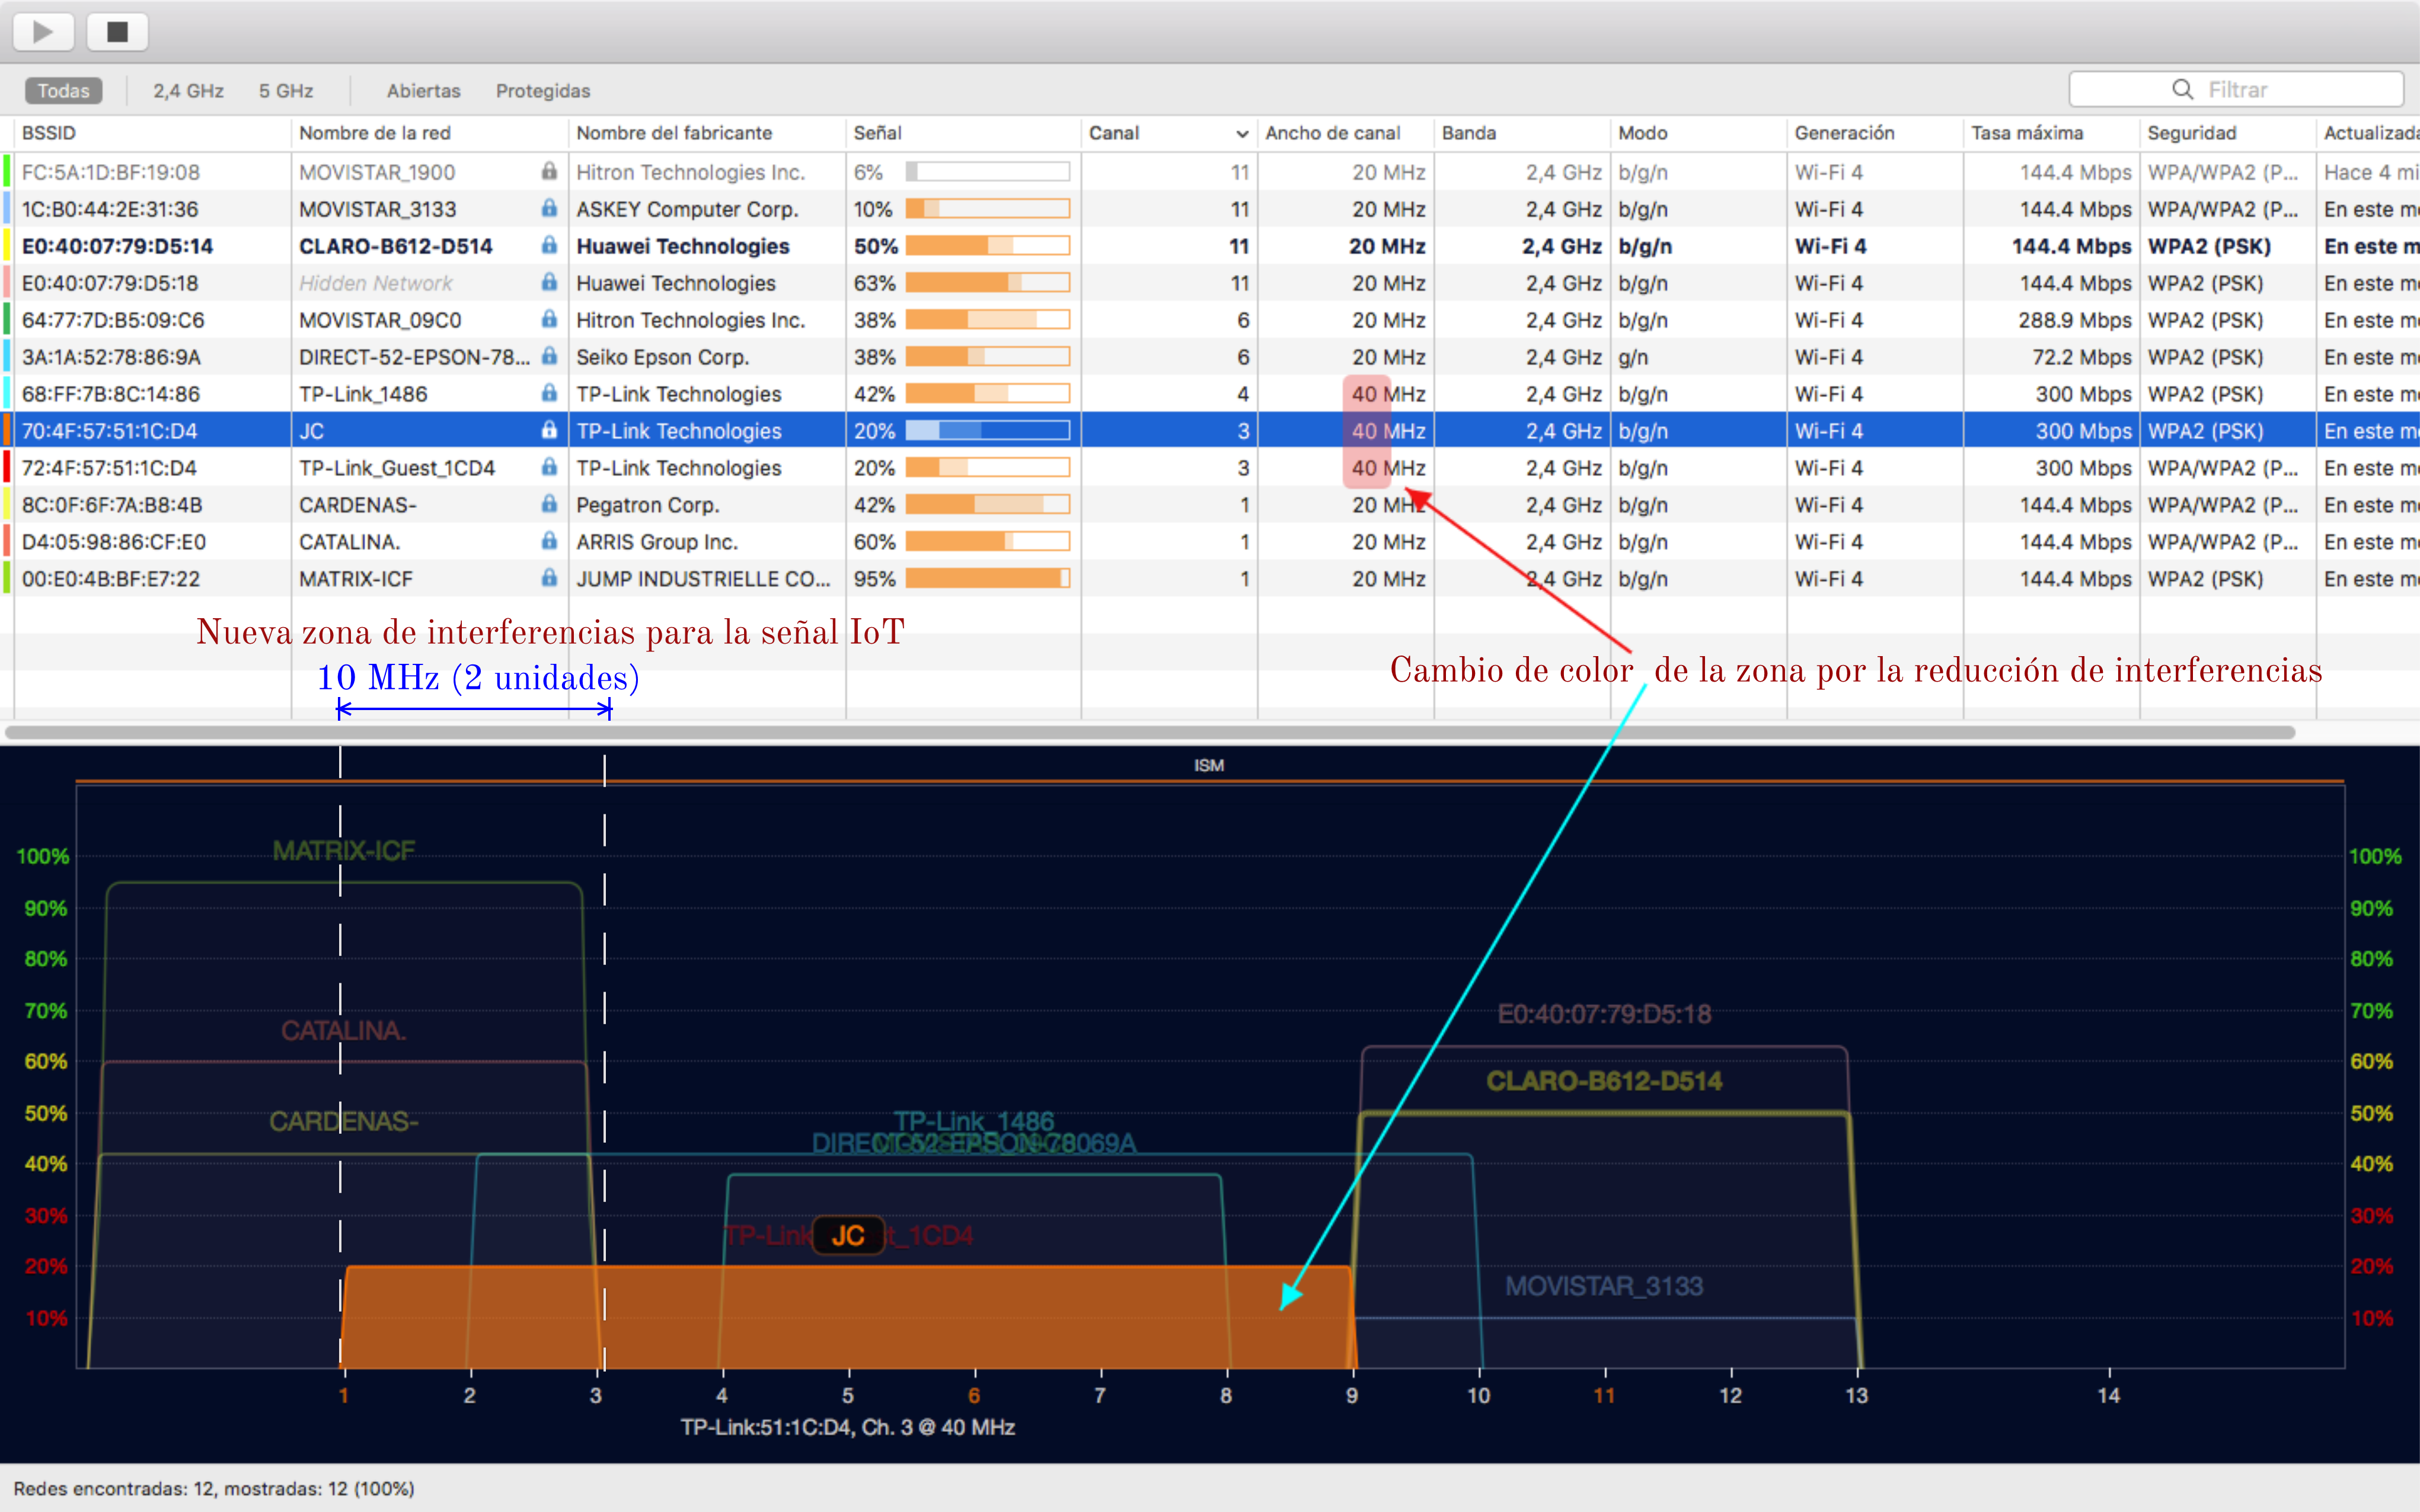
\includegraphics[width=1.5\textwidth]{./Figures/wifi/06.png}
\caption{..... .}
\label{fig:test06}
\end{figure}
\end{landscape} %